A variety of weak mode deformations can exist in the detector even after alignment.
As mentioned previously, these weak modes consist of misalignments which don't affect the $\chi^2$ of the residuals and thus are not handled by the unconstrained alignment algorithm.
In the presence of a weak mode, the description of the detector geometry can still provide efficient and high quality track fits, but there may also be systematic biases in one or more track parameters.
Several weak modes, their impacts on the reconstruction, and the steps taken to eliminate them are detailed in~\cite{2014.alignment-performance-8tev, 2012.alignment-systematics}. 
This section focuses specifically on \emph{sagitta} deformations that result in a bias in the reconstructed track momentum.

These sagitta distortions consist of detector movements orthogonal to the trajectory of the outgoing particle.
The effect on the reconstructed track curvature is different for positively and negatively charged particles, resulting in a charge-antisymmetric bias.
An example of this is illustrated by the curl deformation in Figure~\ref{fig:align_radial_distortion}.

\begin{figure}[htbp]
  \centering
  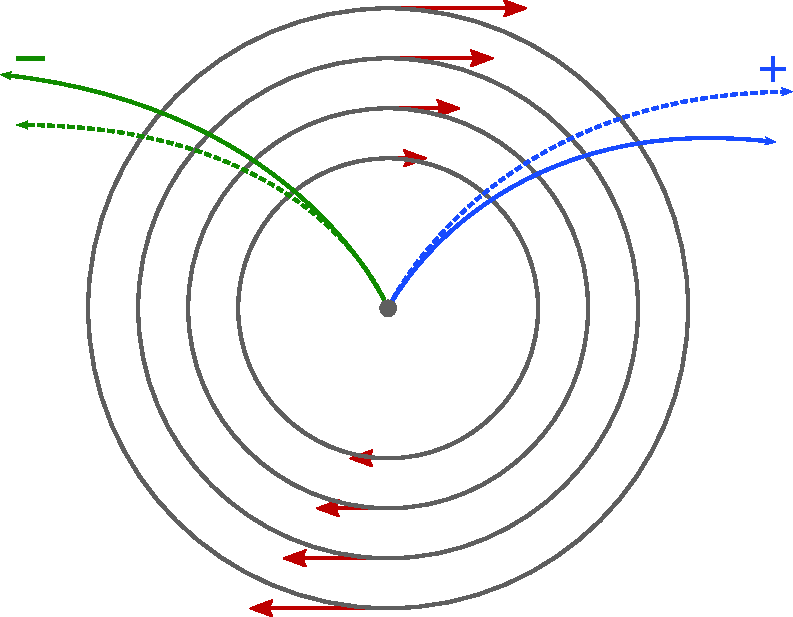
\includegraphics[width=.45\textwidth]{figs/alignment/radial-distortion}
  \caption{Representation of a curl distortion in the detector.  The image represents a cutaway view of the transverse plane of the barrel region.  The deformation is represented by the red arrows, and the impact on the reconstructed positive (blue) and negative (green) tracks are shown.  The dashed lines represent the true particle trajectories, and the solid lines represent the reconstructed trajectories.}
  \label{fig:align_radial_distortion}
\end{figure}

In the plane transverse to ATLAS's magnetic field, outgoing particle tracks form circular arcs.
The sagitta is defined as the distance from the center of this arc to the center of its base, as shown in Figure~\ref{fig:align_sagitta}, and it represents the ``amount of bending'' in the track.
In the case where the sagitta $s$ is considerably smaller than the detector radius $R_0$, which is a valid assumption when working with high momentum tracks, the transverse momentum of a particle of charge $q$ can be written as
\begin{equation}
  \pt \propto q B \frac{R_0^2}{8s}\,,
  \label{eq:align_pt_sagitta}
\end{equation}
where $B$ is the strength of the detector's magnetic field~\cite{2018.alignment-radial-distortions}.
If a sagitta bias is present, the track's transverse momentum shifts by
\begin{equation}
  q/\pt\rightarrow q/\pt+\delta_s ~~~~~\textrm{or}~~~~~ \pt\rightarrow \pt\cdot(1+q\pt\delta_s)^{-1}\,,
  \label{eq:align_pt_sagitta_bias}
\end{equation}
where $\delta_s$ is a universal bias parameter that uniquely defines the deformation~\cite{2012.alignment-systematics}.
Finally, since the reconstructed polar angle does not change under a sagitta deformation, the longitudinal component of the momentum scales along with the transverse component, and an equivalent equation can be written for the total momentum:
\begin{equation}
  p\rightarrow p\cdot(1+q\pt\delta_s)^{-1}\,.
  \label{eq:align_p_sagitta_bias}
\end{equation}

\begin{figure}[htbp]
  \centering
  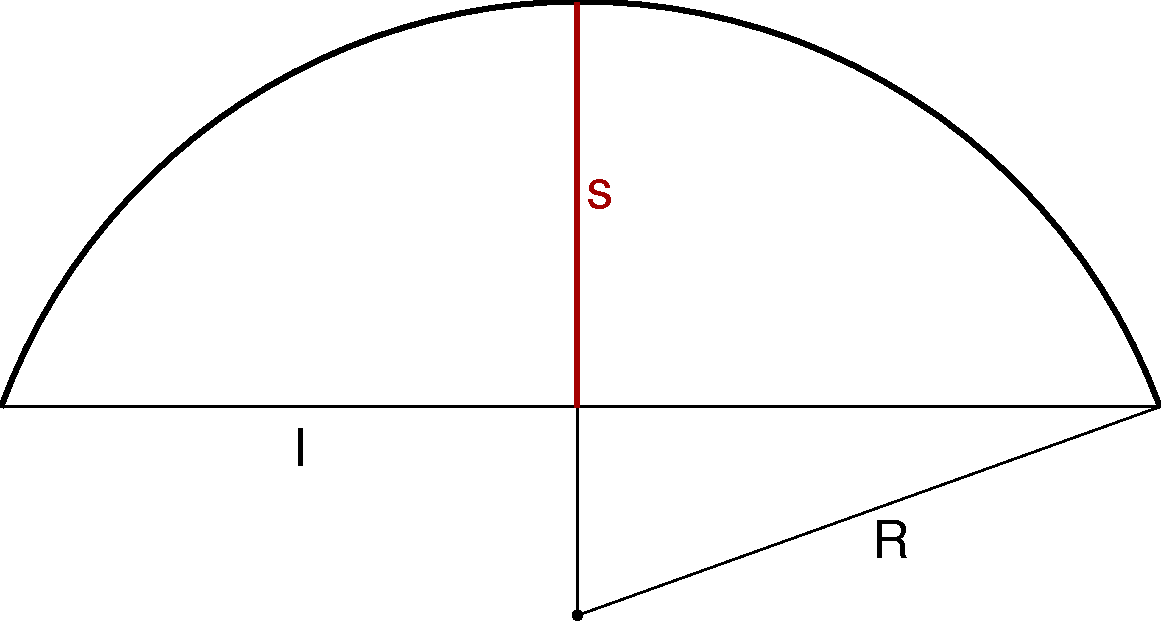
\includegraphics[width=.4\textwidth]{figs/alignment/sagitta}
  \caption{Geometric definition of the sagitta $s$ in relation to the length of the chord $l$ and the radius $R$ of a circular arc.}
  \label{fig:align_sagitta}
\end{figure}

\subsection{Sagitta bias monitoring with electron $E/p$}\label{align:eop}
Since a sagitta bias results in changes in the momenta of particle tracks as measured by the ID, they can be identified using independent measurements from other systems in the detector.
One such method involves using the energy-momentum ratio of electrons ($E/p$).
Since the electron's energy is measured in ATLAS's calorimeter systems, it is not sensitive to any sagitta bias that may exist in the ID and in the corresponding measurement of the track momentum.
Under the assumption that the calorimeter response is independent of the charge of incoming particles, a charge-dependent momentum bias in the ID will manifest as a difference in the $E/p$ ratio for electrons and positrons.%\footnote{For the remainder of this section, electrons and positrons will collectively be referred to as ``electrons'' unless explicitly noted.}.

In the presence of a sagitta bias, the momentum will change according to Equation~\ref{eq:align_p_sagitta_bias} and the average measured $\eop$ can be written as
\begin{equation}
  \eop^{\pm}\rightarrow\eop^{\pm}\pm\langle\et\rangle\delta_s\,,
\end{equation}
where the approximation $\pt\approx\et$ is used.
Assuming that $\eop^+ = \eop^-$ in the absence of a bias, the sagitta bias parameter can be solved for:
\begin{equation}
  \delta_s = \frac{\eop^+ - \eop^-}{2\langle\et\rangle}\,.
\label{eq:align_eop_sagitta}
\end{equation}
If the kinematic selections for electrons and positrons are identical, the energy scale of the calorimeter will not factor into the $\eop$ difference; however, it will affect $\langle\et\rangle$, which would scale the measured $\delta_s$.
This is expected to be a small effect, as the energy scale for electrons has been measured at $13\tev$ with uncertainties on the per-mil level across the entire detector~\cite{2016.electron-photon-calibration}.

\subsubsection{Measuring $\eop$}
The $E/p$ ratio is measured using electrons and positrons from $Z\rightarrow ee$ events in order to obtain a high purity sample of candidate particles.
They are required to pass a basic selection criteria to ensure they are well measured in both the ID and the calorimeters:
\begin{itemize}
  \item $\et > 25\gev$
  \item $|\eta| < 2.47$, excluding the calorimeter's barrel-to-endcap transition region in $1.37<|\eta|<1.52$
  \item Pass the \tt{MediumLH} identification working point detailed in Section~\ref{detector:electron_reconstruction}
  \item Pass a selection of quality cuts, including a requirement that the electron be identified using cluster information in the calorimeter %author == 1 is cluster based only, author == 3 is cluster and track-based
  \item The associated track must have at least one hit in the IBL, three in the Pixel detector, and five in the SCT detector.
\end{itemize}
Events containing exactly two opposite-charge electrons passing this selection with an invariant mass within $30\gev$ of the $Z$ boson mass are then used for the $E/p$ calculation.

Since the size of the sagitta bias $\delta_s$ is not expected to be constant across the entire detector, a two-dimensional rectangular grid is constructed binned in detector $\eta$ and $\phi$.
From the selected events, separate distributions of $E/p$ are made for electrons and positrons within each bin.
Each distribution is fit with Crystal Ball function\footnote{The Crystal Ball function is a probability density function consisting of a Gaussian core and a power-law tail.}, and the peak of the distribution is taken as the value of $\eop$.
If there is no bias on the track momentum in the bin, the peaks for electrons and positrons should agree.
Example $E/p$ distributions including the Crystal Ball fits are shown in Figure~\ref{fig:alignment_eop_fit}.

It is important to emphasize that deviations from one in the \emph{ratio} of $\eop^+$ to $\eop^-$ points to a potential momentum biases.
The value of $\eop$ itself is not expected to equal one exactly, as the track momentum on average tends to be slightly lower than the energy measurement in the calorimeter.
This is due to the fact that if the electron were to radiate a photon, its momentum would change slightly, while it is likely that both the electron and the emitted photon would leave energy deposits near each other in the calorimeter and be reconstructed into the same object. 

\begin{figure}[htbp]
  \centering
  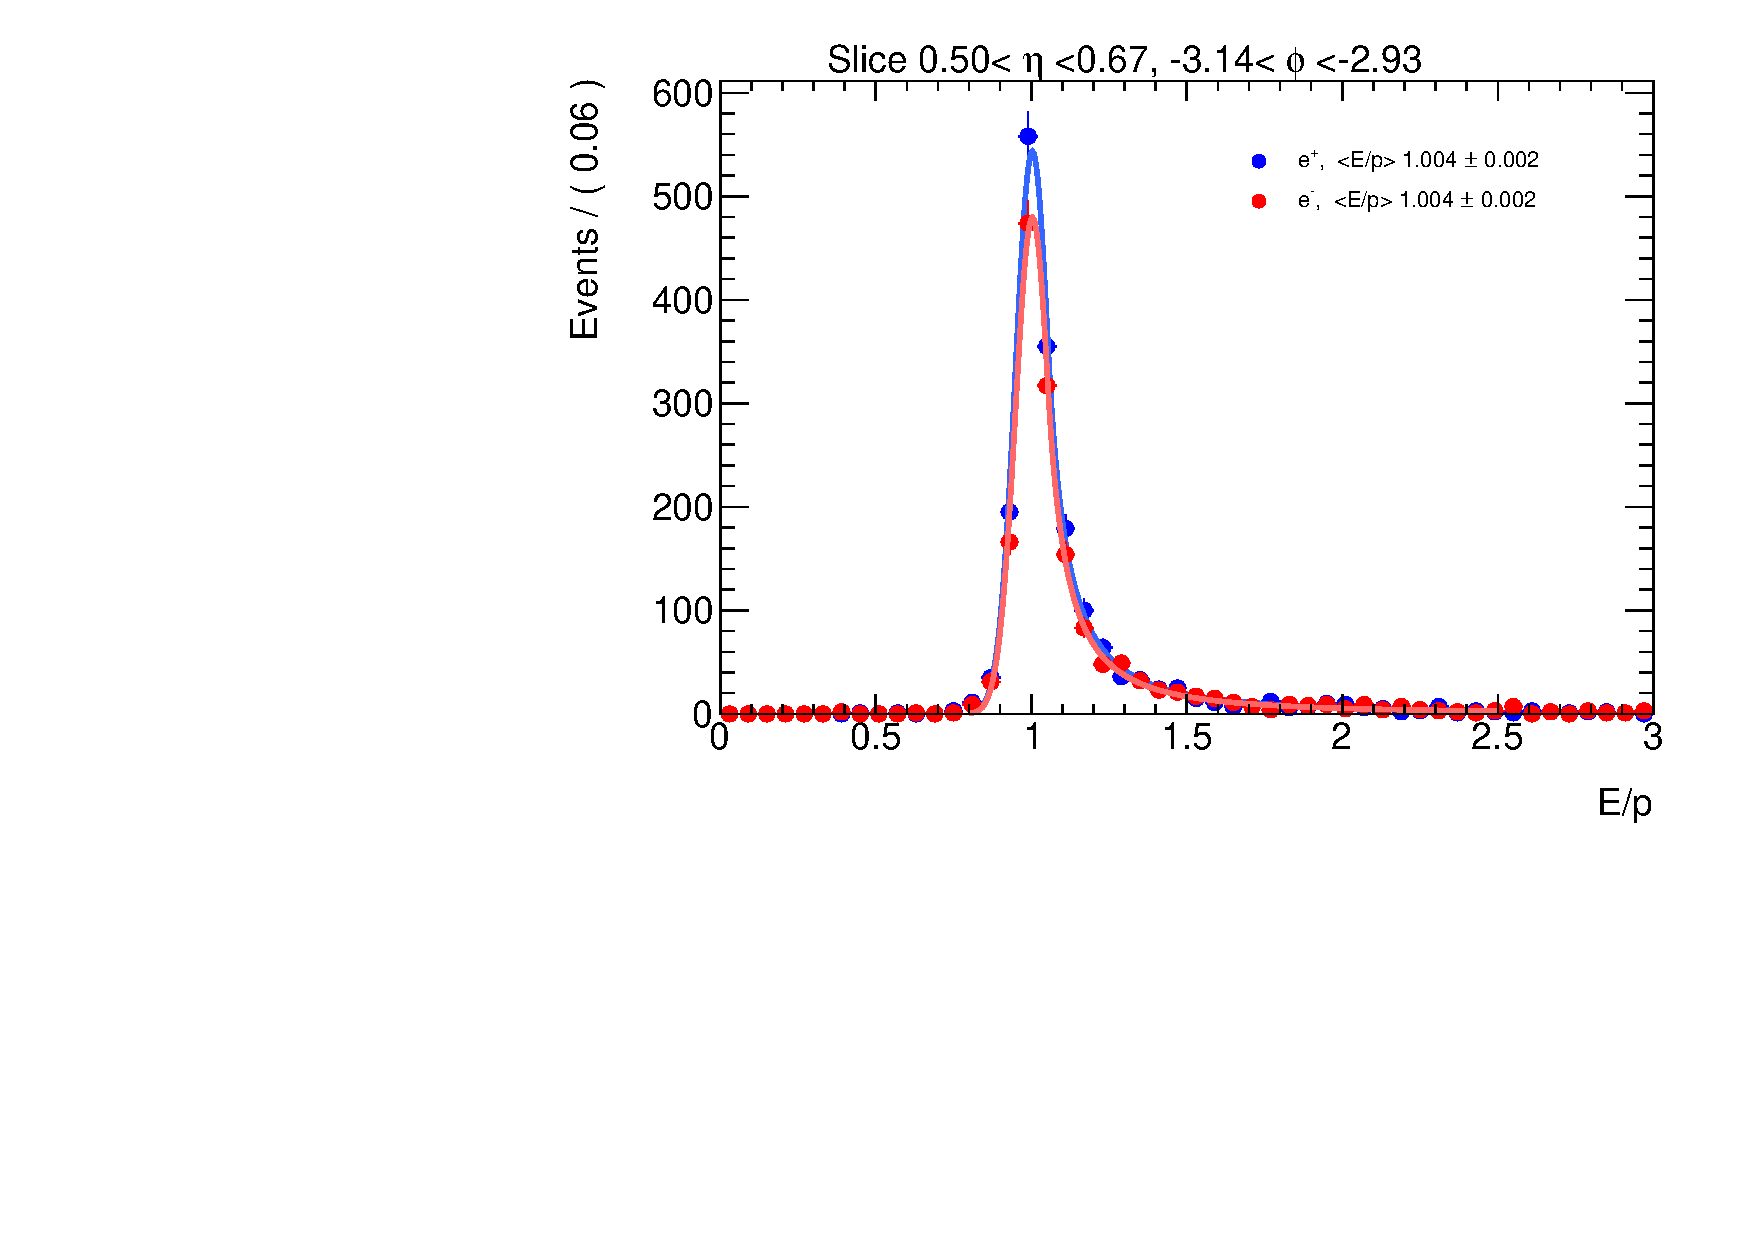
\includegraphics[width=.48\textwidth]{figs/alignment/eop/eop_fit_nobias}
  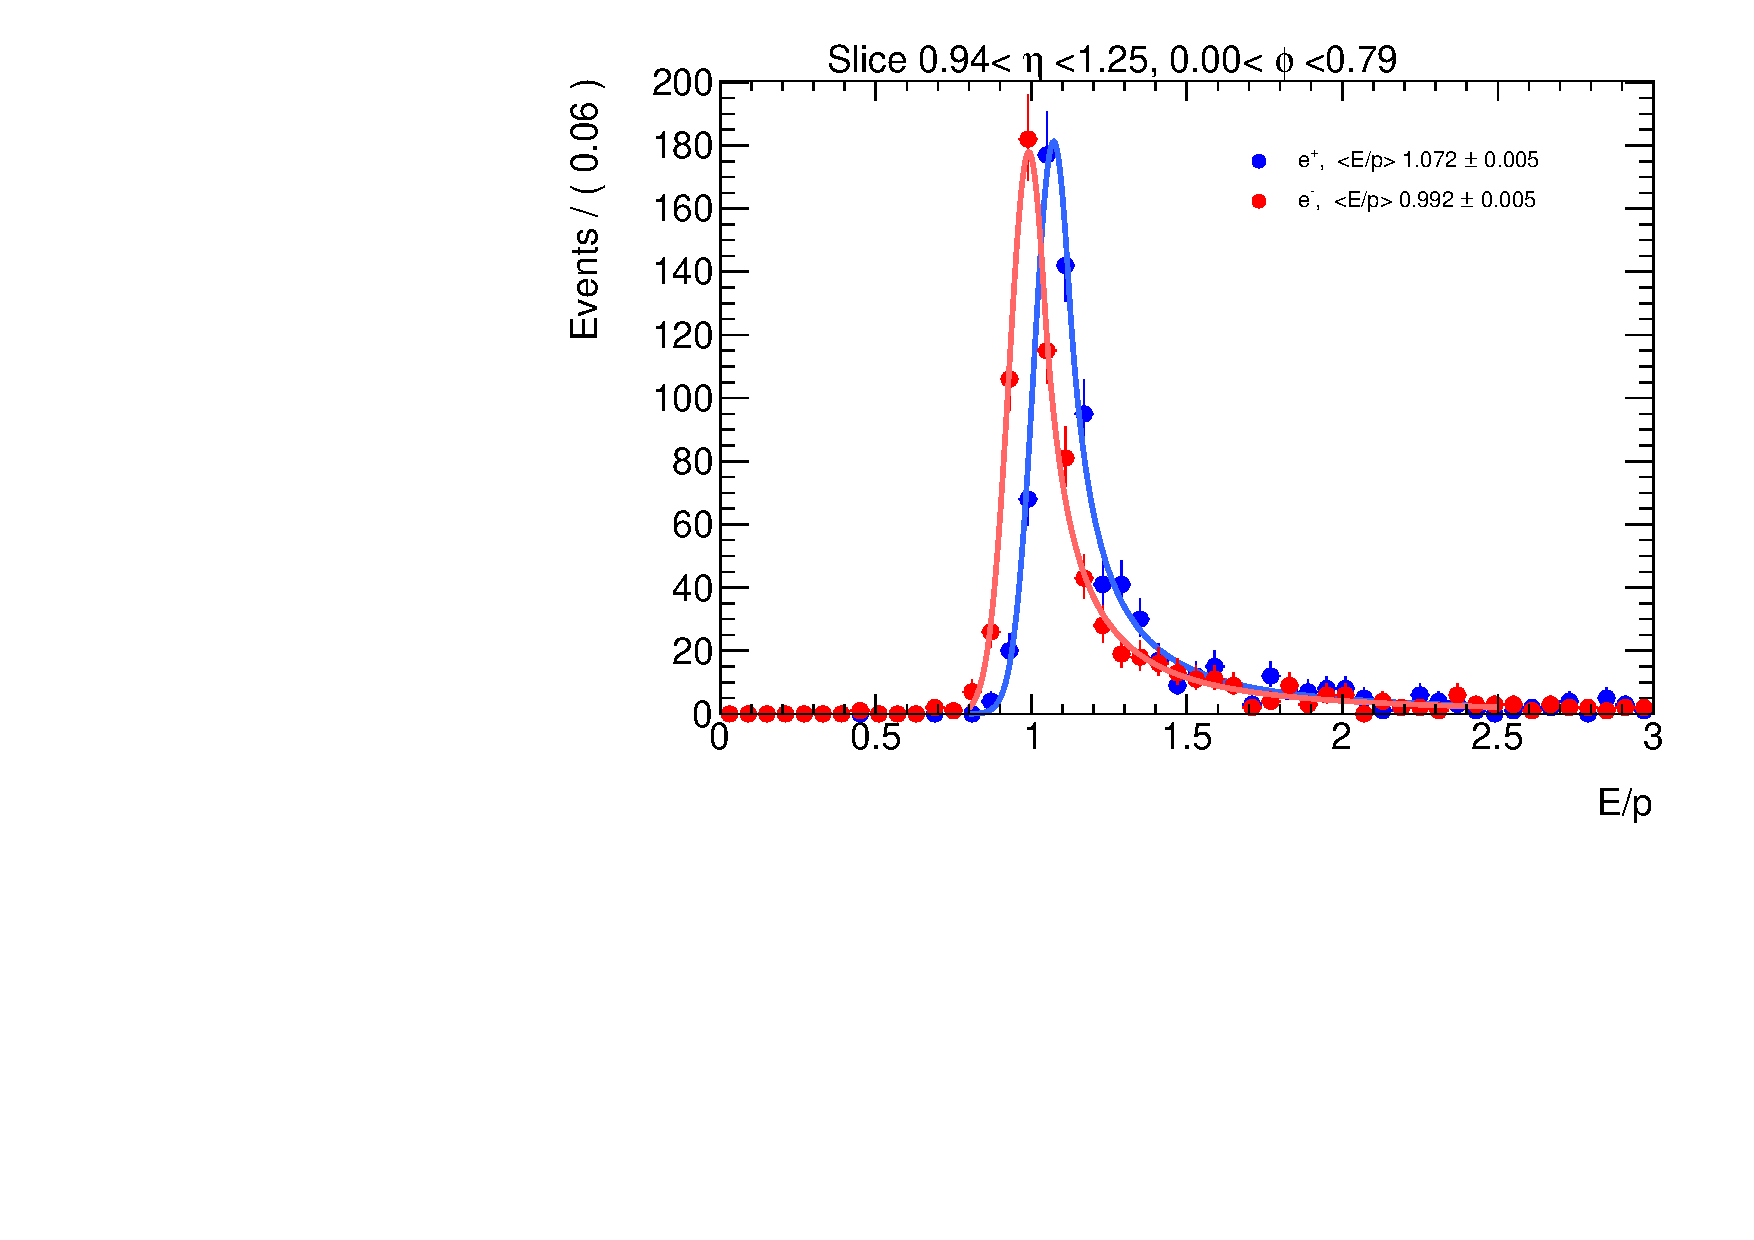
\includegraphics[width=.48\textwidth]{figs/alignment/eop/eop_fit_bias}
  \caption{$E/p$ distributions of electrons and positrons in two different $\eta$-$\phi$ bins of the detector.  The left hand plot is taken from a region with no momentum bias where $\eop^+ = \eop^-$, while the right hand plot shows an 8\% disagreement in $\eop$ between electrons and positrons.}
  \label{fig:alignment_eop_fit}
\end{figure}

Once the $\eop^\pm$ distributions in each $\eta$-$\phi$ bin have been extracted from the fits, a two dimensional map of $\delta_s$ can be constructed using Equation~\ref{eq:align_eop_sagitta}.
The map gives an overview of sagitta biases that may be present in the detector, and can be used by the alignment algorithm to reduce the bias in the next iteration.
In this case, the tracks fed to the alignment have their momenta corrected according to
\begin{equation}
q/p_{\textrm{corr}} = q/p_{\textrm{reco}}(1-q\pt\delta_s)\,,
\end{equation}
where $p_{\textrm{reco}}$ is the reconstructed momentum of the track~\cite{2012.alignment-systematics}.
The corrected momentum is then constrained in the alignment.

\subsubsection{Results in $13\tev$ data}
The $E/p$ method has been used to monitor sagitta biases in the detector several times over the course of Run 2.
During this time, it has primarily served as an independent cross-check to a second method using $Z\rightarrow\mu\mu$ events~\cite{2012.alignment-systematics}.
The $Z\rightarrow\mu\mu$ method identifies individual track momentum biases through shifts in the reconstructed $Z$ mass, which leaves it relatively insensitive to global sagitta biases.
For this reason, the sagitta bias maps produced using this technique are normalized to those from the $E/p$ method before being used to constrain the alignment. 
The results of two implementations of the $E/p$ method are presented here.
\begin{enumerate}
\item The first follows the end-of-year reprocessing of the entire ATLAS 2016 data set. % at \com{13}.
Two sets of alignment constants are compared: the \emph{prompt} alignment, which was derived shortly after each run was recorded, and the \emph{reprocessed} alignment.
The maps of the sagitta bias in each alignment calculated using the $E/p$ method are shown in Figure~\ref{fig:alignment_2016_sagitta_map}, and the comparison of the $\eta$ projection of the maps is shown in Figure~\ref{fig:alignment_2016_sagitta_projection}.
\item The second uses the 2017 data after reprocessing, and compares the effects of multiple iterations of the $E/p$ method.
In each iteration, the momenta of the electrons and positrons are corrected according to Equation~\ref{eq:align_p_sagitta_bias} using the value of $\delta_s$ computed in the previous iteration, and a new sagitta bias map is calculated.
If the method is indeed characterizing the sagitta biases correctly, the corrections should converge quickly.
The initial sagitta bias map is compared to the map after two such iterations in Figure~\ref{fig:alignment_2017_sagitta_map}, and the sagitta bias projected along $\eta$ for each iteration is shown in Figure~\ref{fig:alignment_2017_sagitta_projection}.
Indeed, after just two iterations, $\delta_s$ is consistent with zero in nearly all bins.
\end{enumerate}

\begin{figure}[htbp]
  \centering
  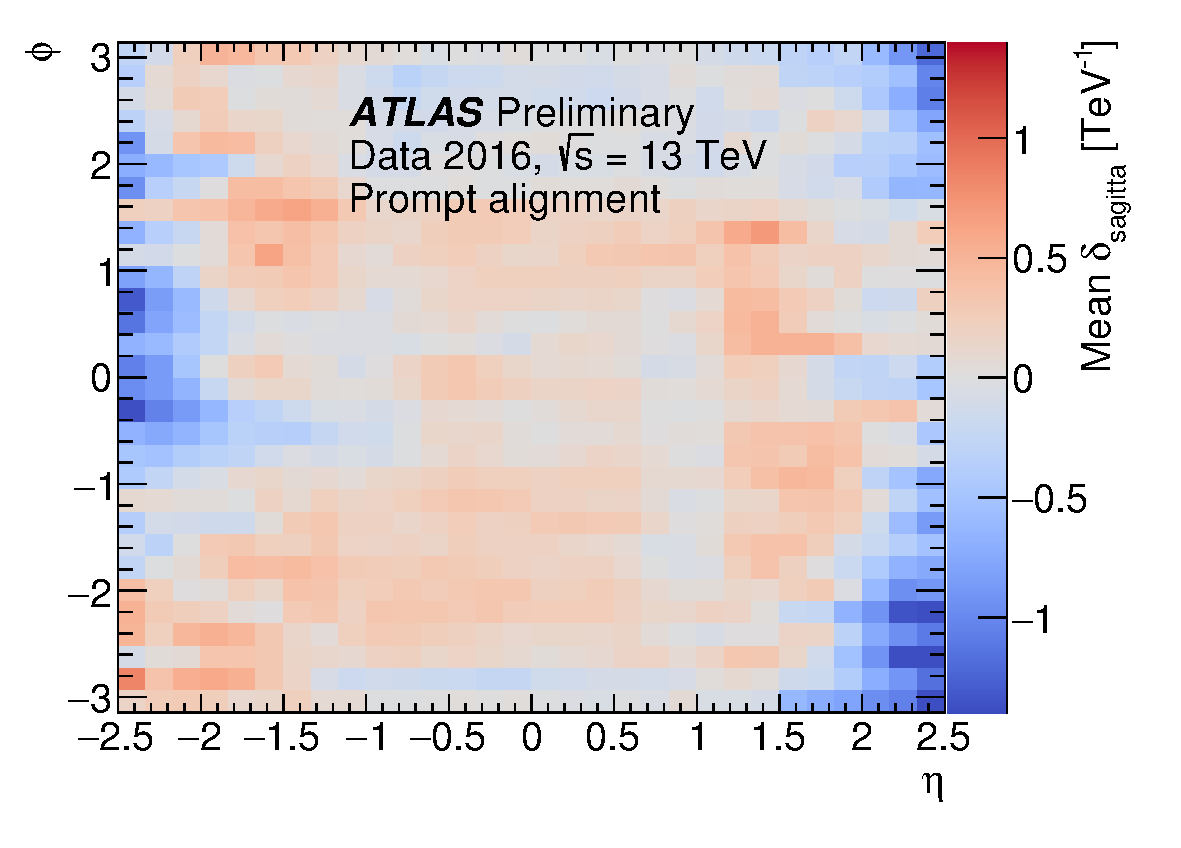
\includegraphics[width=.48\textwidth]{figs/alignment/eop/public_plot_map_prompt}
  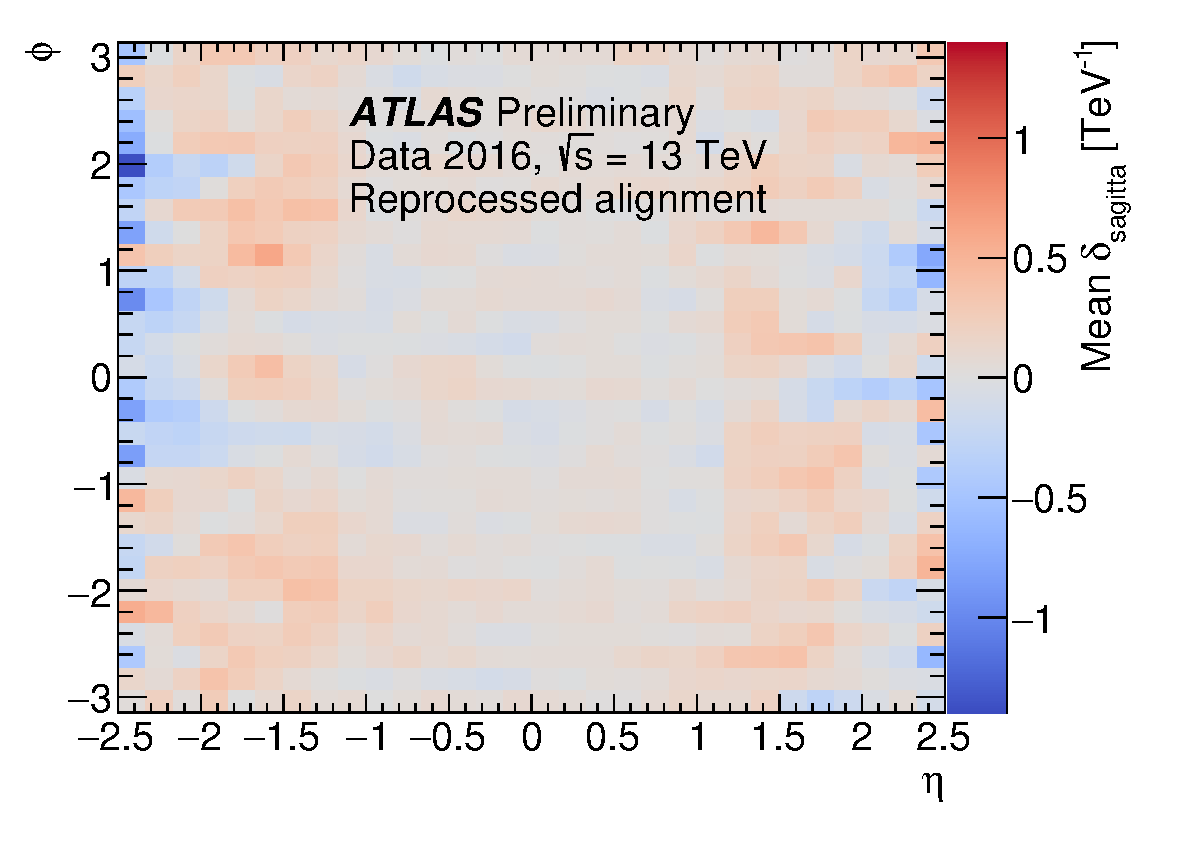
\includegraphics[width=.48\textwidth]{figs/alignment/eop/public_plot_map_reprocessed}
  \caption{Sagitta bias in the \com{13} data collected by ATLAS in 2016 as a function of $\eta$ and $\phi$ for the prompt (left) and reprocessed (right) alignments using the $E/p$ method.}
  \label{fig:alignment_2016_sagitta_map}
\end{figure}

\begin{figure}[htbp]
  \centering
  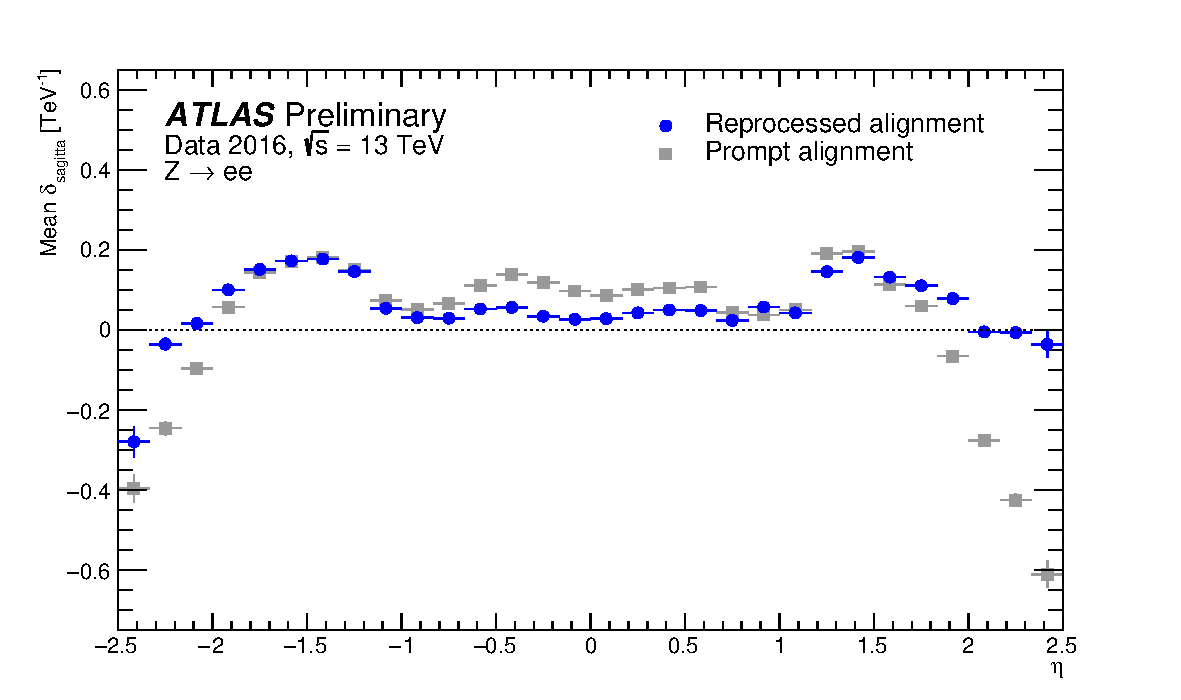
\includegraphics[width=.6\textwidth]{figs/alignment/eop/public_plot_projection}
  \caption{Sagitta bias in the \com{13} data collected by ATLAS in 2016 projected along $\eta$ for the prompt (gray) and reprocessed (blue) alignments using the $E/p$ method.}
  \label{fig:alignment_2016_sagitta_projection}
\end{figure}

\begin{figure}[htbp]
  \centering
  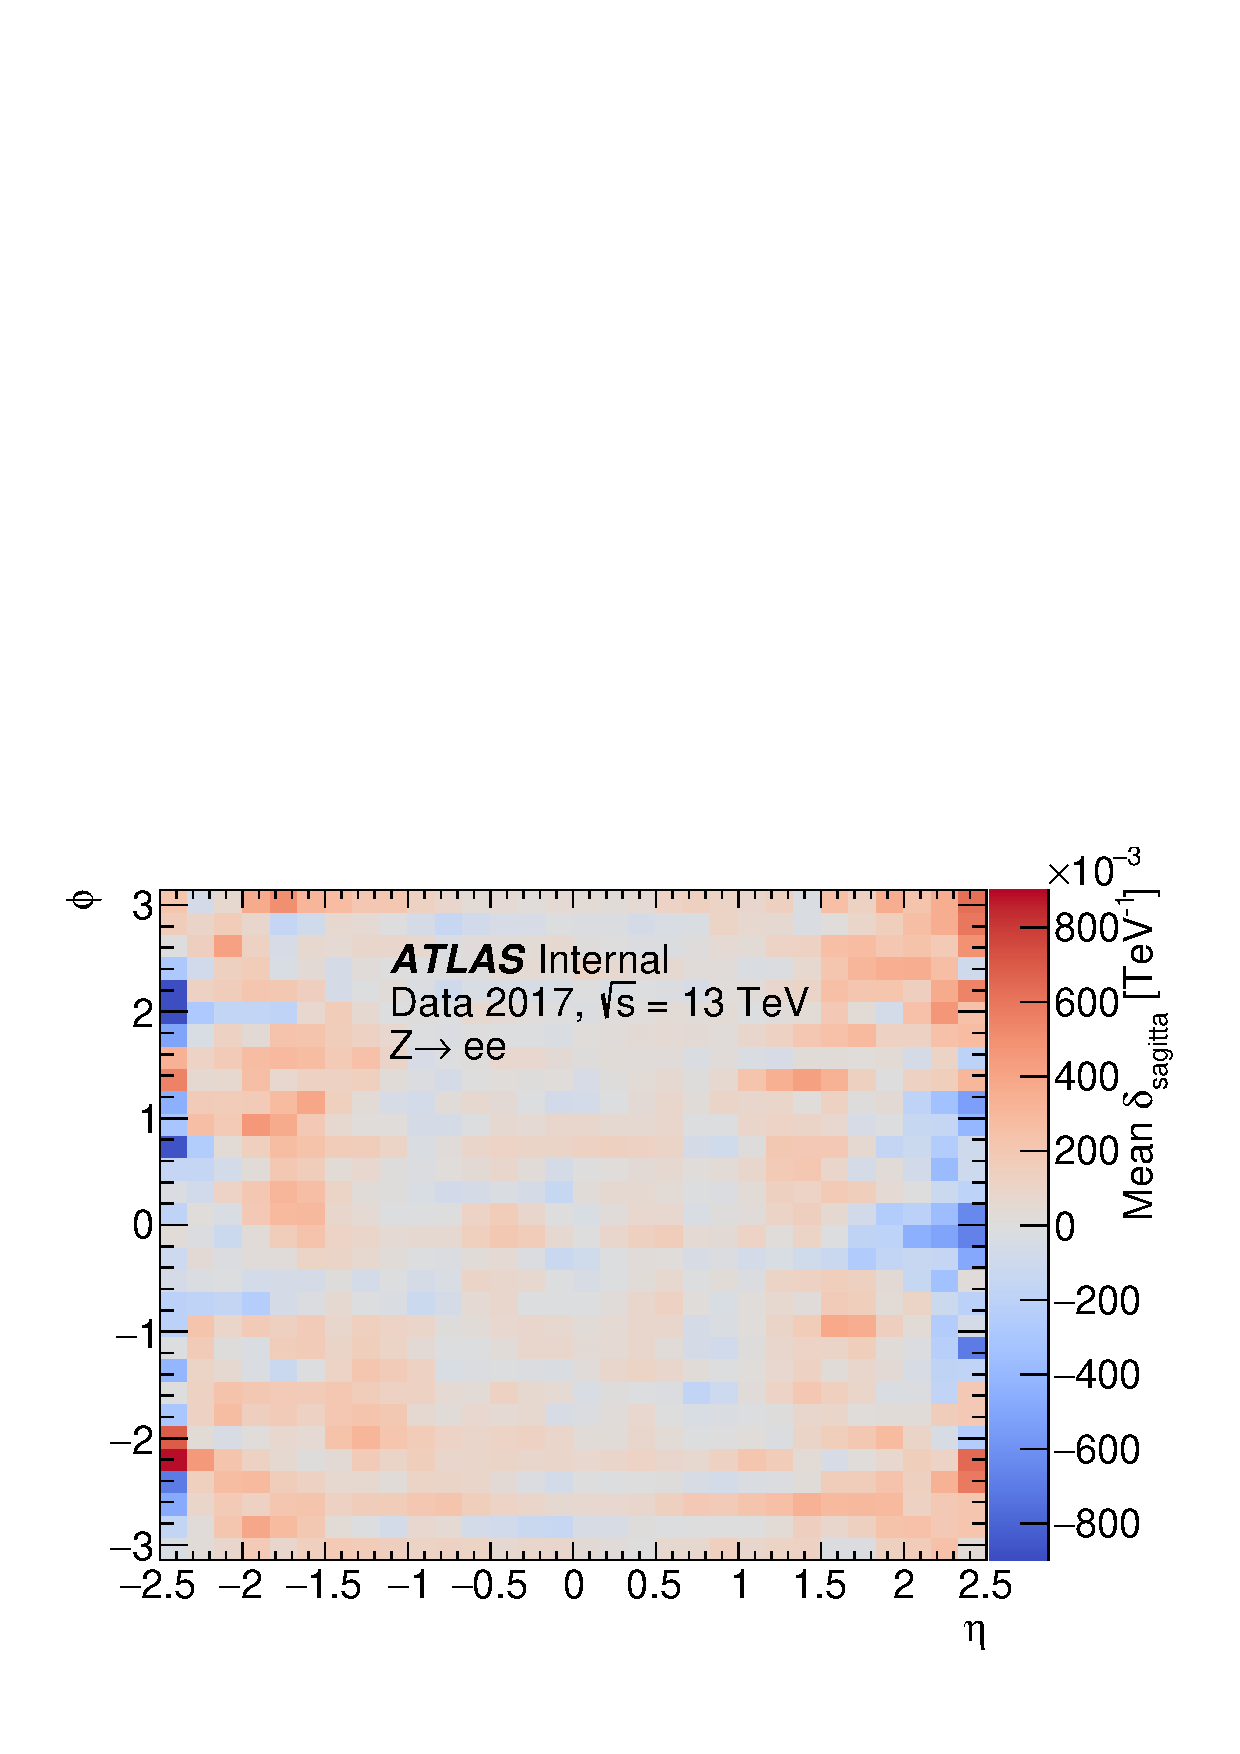
\includegraphics[width=.48\textwidth]{figs/alignment/eop/sagitta_2017}
  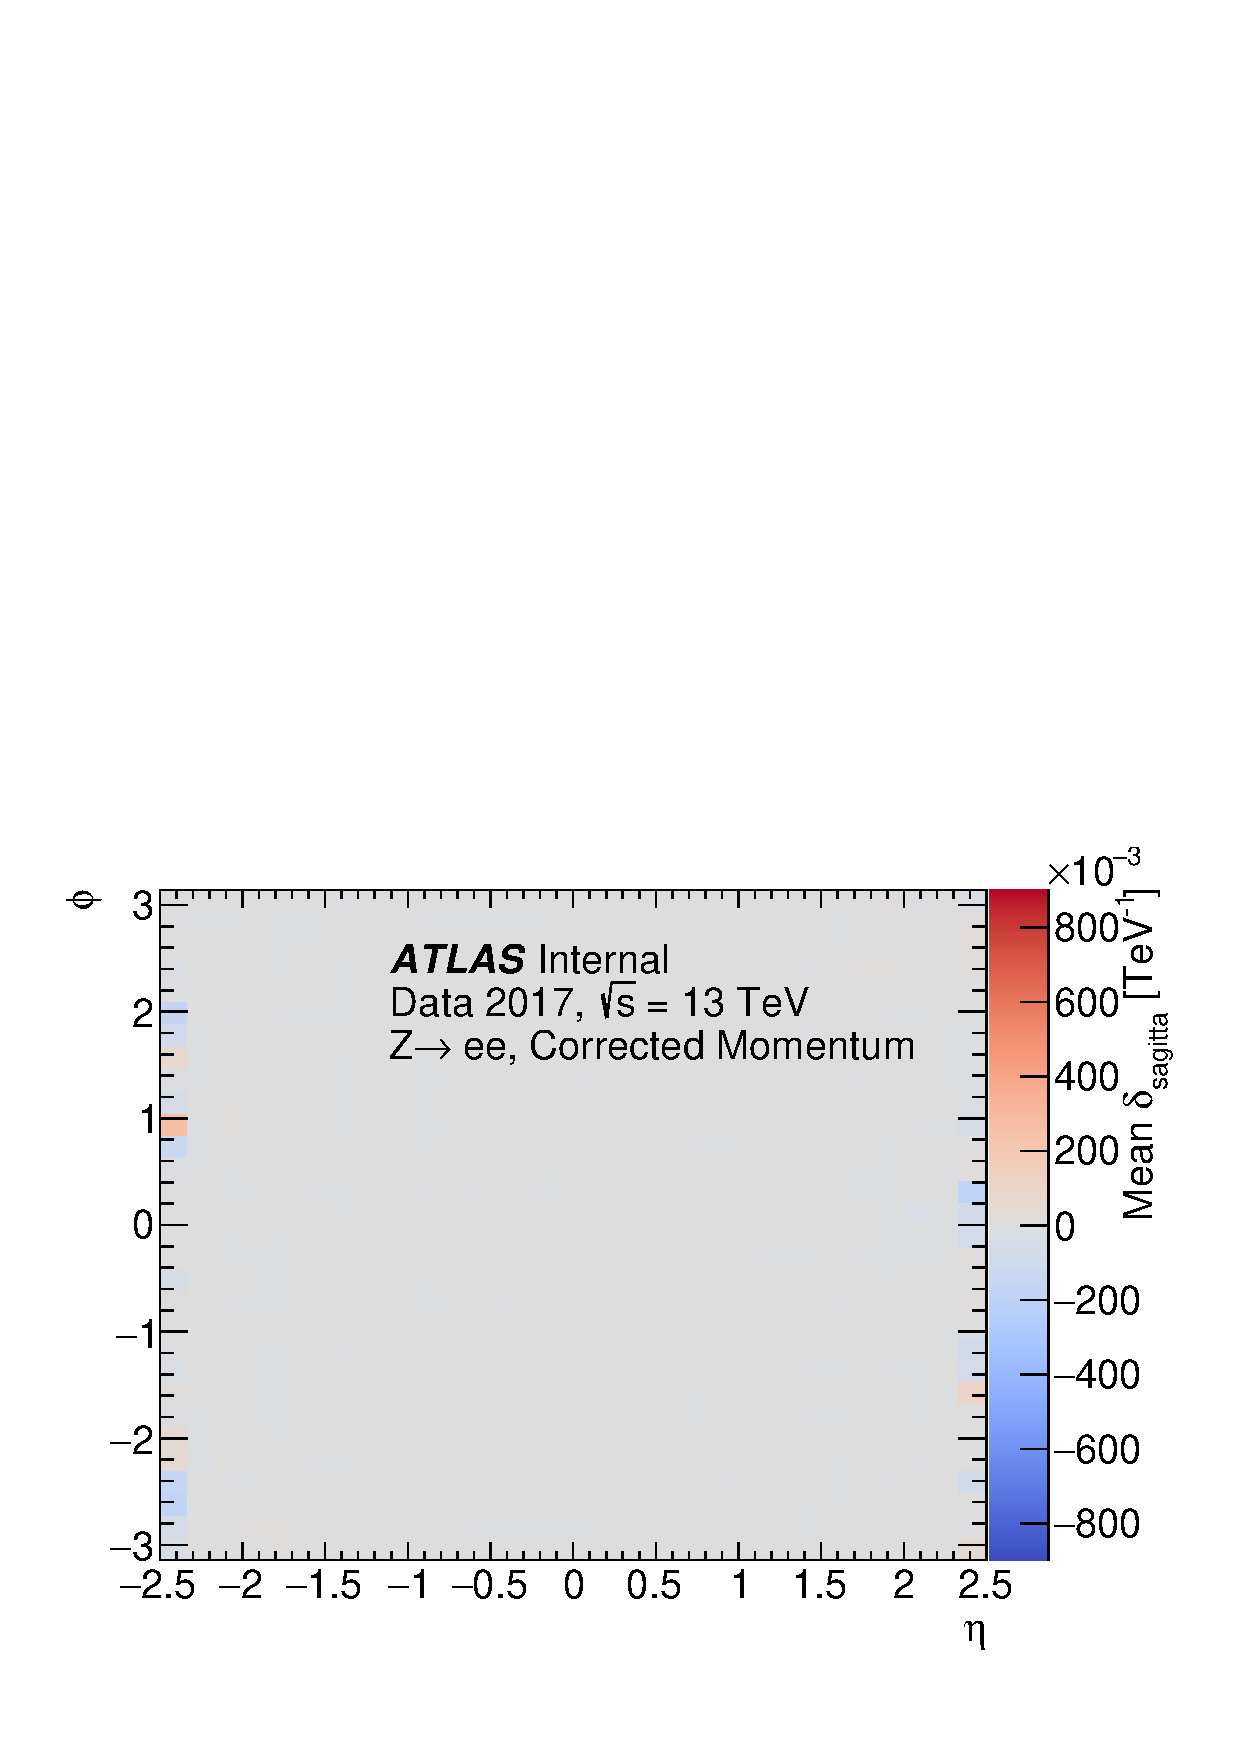
\includegraphics[width=.48\textwidth]{figs/alignment/eop/sagitta_2017_Iter2}
  \caption{Sagitta bias in the \com{13} data collected by ATLAS in 2017 as a function of $\eta$ and $\phi$ in reconstructed electrons (left) and after two iterations of momentum corrections (right) from the $E/p$ method.}
  \label{fig:alignment_2017_sagitta_map}
\end{figure}

\begin{figure}[htbp]
  \centering
  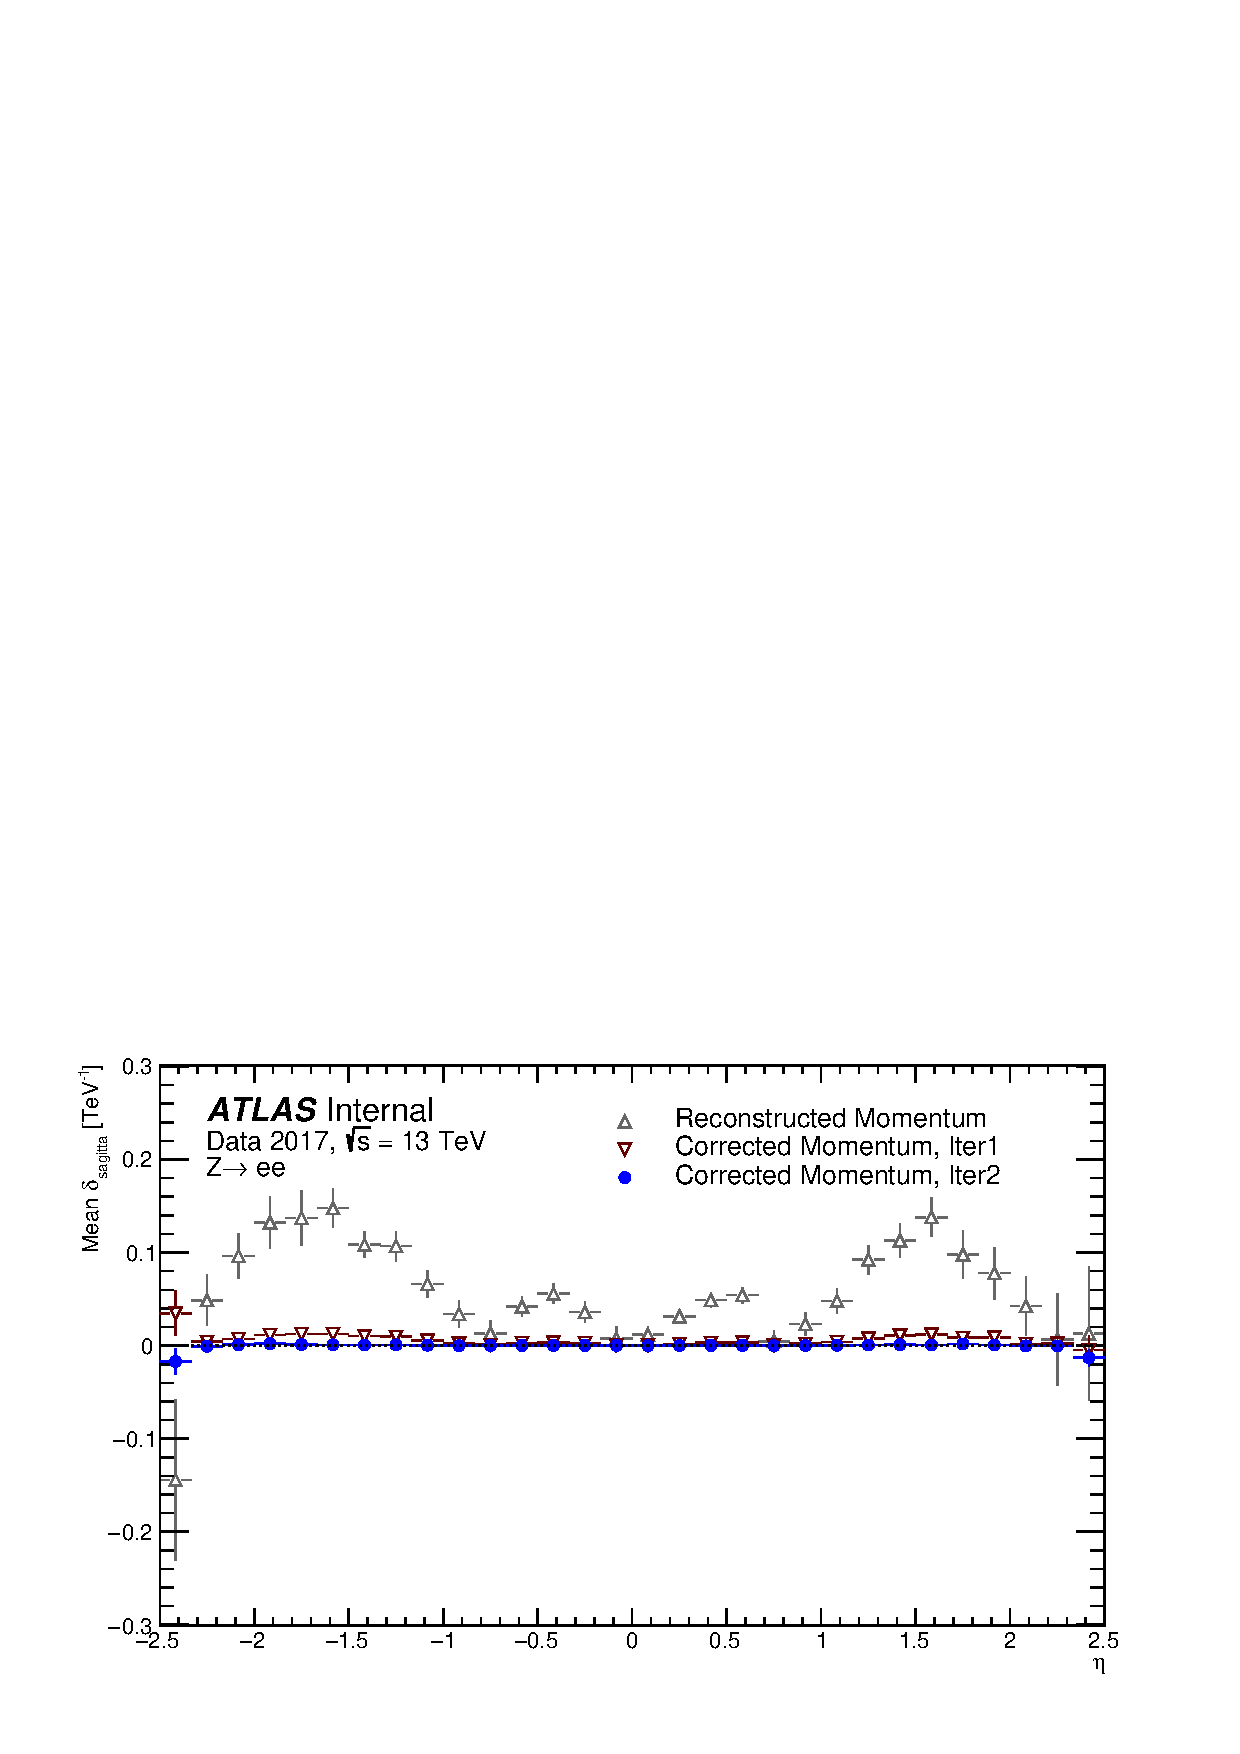
\includegraphics[width=.6\textwidth]{figs/alignment/eop/sagitta_2017_projection}
  \caption{Sagitta bias in the \com{13} data collected by ATLAS in 2017 projected along $\eta$ in reconstructed electrons (gray) and after one (red) and two (blue) iterations of momentum corrections from the $E/p$ method.}
  \label{fig:alignment_2017_sagitta_projection}
\end{figure}
